\documentclass[11pt,a4paper]{article}

\usepackage{amsmath,amssymb,amsthm}
\usepackage{graphicx}
\usepackage{natbib}
\newtheorem{lemma}{Lemma}
\setcitestyle{aysep={}}
\usepackage[margin=2.5cm]{geometry}

\title{Likelihood targets of a nested ensemble Kalman filter}
\author{Andrew Golightly\\
Department of Mathematical Sciences, Durham University}
\date{15 October 2026}

\begin{document}
\maketitle

\begin{abstract}
State-space models with a static parameter have an observed-data likelihood that integrates out a latent Markov process. Nested particle filters for the parameter become expensive as the observation dimension grows. Replacing each likelihood increment by an ensemble Kalman forecast changes the posterior, and replacing that forecast by a nearest-neighbour prediction changes it again. These are different errors. We separate them. The plain filter targets the ensemble Kalman posterior. The nearest-neighbour weight targets the surrogate posterior. A Rao-Blackwellised weight puts the true observation density back, whilst the forecast stays Gaussian. If the observation density is already that Gaussian density, the two weights agree. On a Lotka--Volterra diffusion, with prey observed under a Gaussian density whose variance equals the latent prey, we compare the plain filter, the Rao-Blackwellised filter and bootstrap sequential Monte Carlo squared. The plain filter lies 0.0586 and 0.0354 below the bootstrap filter on the log predation coefficient and the log predator death rate. Neither gap exceeds its standard error, so the shift is unresolved. No bound between the surrogate posterior and the ensemble Kalman posterior was obtained.
\end{abstract}

\noindent\textbf{Keywords:} Lotka--Volterra model, Rao-Blackwellisation, sequential Monte Carlo, state-space model, surrogate likelihood

\section{Introduction}

State-space models are used when a latent Markov process is observed with noise and a static parameter governs the transition and the observation. The observed-data likelihood is an integral over the latent path, and that integral is rarely available in closed form. Sequential Monte Carlo squared (SMC2) propagates a cloud of parameter particles, reweights them by a particle-filter estimate of each likelihood increment, and moves them with a particle Metropolis--Hastings kernel when the effective sample size falls \citep{chopin2012}. The variance of that estimate grows with the length of the series and, more sharply, with the observation dimension.

The ensemble Kalman filter replaces the forecast distribution by a Gaussian distribution whose mean and covariance are the sample moments of an ensemble, and it updates the ensemble with a Kalman shift. The likelihood contribution is then the Gaussian marginal of that forecast. It is not unbiased for the true likelihood. \citet{golightly2026} place this contribution inside the SMC2 recursion. The resulting nested ensemble Kalman filter targets the parameter posterior induced by the ensemble Kalman likelihood, which we denote \(\hat{\pi}_{\mathrm{enkf}}\), rather than the exact posterior \(\pi_t\).

For a nonlinear or non-Gaussian observation the same construction replaces the observation density by a linear Gaussian approximation before the ensemble update. The plain filter still targets \(\hat{\pi}_{\mathrm{enkf}}\), now under that approximation. A Rao-Blackwellised weight puts the true observation density back into the increment, while the forecast remains Gaussian, and targets a different posterior, which the source paper denotes \(\tilde{\pi}_{\mathrm{enkf}}\). Vanilla SMC2, with a bootstrap proposal, targets \(\pi_t\). Separately, the nearest-neighbour surrogate that \citet{golightly2026} use to screen a Metropolis--Hastings proposal can be used as the incremental weight itself. That choice defines a further posterior, which we denote \(\pi_{\mathrm{knn}}\). A screen that is corrected by the ensemble Kalman likelihood leaves \(\hat{\pi}_{\mathrm{enkf}}\) invariant. A weight that is the surrogate does not.

These are two errors, and a comparison that jumps from \(\pi_{\mathrm{knn}}\) to \(\pi_t\) mixes them. The first error is the ensemble Kalman likelihood against the true likelihood, hence \(\hat{\pi}_{\mathrm{enkf}}\) against \(\pi_t\). The second is the nearest-neighbour prediction against the ensemble Kalman likelihood, hence \(\pi_{\mathrm{knn}}\) against \(\hat{\pi}_{\mathrm{enkf}}\). On the Lotka--Volterra diffusion in Section~5.2 of \citet{golightly2026}, the observation is Gaussian with variance equal to the latent prey state. That paper reports that the plain filter shifts the posterior means of \(\theta_2\) and \(\theta_3\) because the observation variance is replaced by a function of the forecast mean, and that the Rao-Blackwellised filter reduces the discrepancy at greater cost. The distance between \(\pi_{\mathrm{knn}}\) and \(\hat{\pi}_{\mathrm{enkf}}\) is not bounded there.

Our contribution is to separate the two errors and to compare the three targets on that nonlinear observation model. (i)~The plain nested filter targets \(\hat{\pi}_{\mathrm{enkf}}\). The nearest-neighbour incremental weight targets \(\pi_{\mathrm{knn}}\), and we do not treat those posteriors as the same object. (ii)~When the true observation density equals the linear Gaussian density inside the filter, the Rao-Blackwellised weight equals the ensemble Kalman weight. The identity is specific to that case. (iii)~On the Lotka--Volterra observation we compare the plain filter, the Rao-Blackwellised filter and bootstrap SMC2, under a reduced design that is stated as such. A bound on the distance between \(\pi_{\mathrm{knn}}\) and \(\hat{\pi}_{\mathrm{enkf}}\) was not obtained. The paper reports the diagnostic that was fixed before any output was seen. A faster neighbour search, a kernel chosen by time, and a finite-difference proposal were examined in an earlier pilot and are not contributions here.

The identity is checked on a scalar Ornstein--Uhlenbeck diffusion with a known Kalman likelihood, at a smaller particle count and a shorter series than Section~5.1 of \citet{golightly2026}. The nonlinear comparison uses one prey series from the Lotka--Volterra diffusion, with fewer parameter particles and fewer algorithm replicates than Section~5.2, and without the particle Markov chain Monte Carlo gold standard used there. No epidemic series is analysed. \citet{temfack2026} already study a nested ensemble scheme for epidemic incidence.

The remainder of this paper is organised as follows. Section~\ref{sec:related} describes the neighbouring algorithms and which posterior each one targets. Section~\ref{sec:methods} separates the two errors and records the identity. Section~\ref{sec:sim} reports the identity check and the Lotka--Volterra comparison, and Section~\ref{sec:disc} discusses what those runs support and what remains open.

\section{Related work}
\label{sec:related}

The algorithms in this section all propagate information about a static parameter of a state-space model, or they are the constructions with which the nested filter is easily confused. They do not share a parameter target. Table~\ref{tab:targets} records the distinction that the rest of the paper uses. The nearest-neighbour row is the target defined in Section~\ref{sec:methods}. The other rows are the algorithms as published.

\begin{table}[htbp]
\centering
\caption{Parameter targets of the neighbouring schemes. The exact posterior is \(\pi_t\). The ensemble Kalman posterior is the posterior induced by the ensemble Kalman likelihood. Citations for the rows are \citet{chopin2012}, \citet{drovandi2022}, \citet{katzfuss2018}, \citet{golightly2026} and \citet{temfack2026}.}
\label{tab:targets}
\small
\begin{tabular}{>{\raggedright\arraybackslash}p{3.15cm}>{\raggedright\arraybackslash}p{4.15cm}>{\raggedright\arraybackslash}p{4.35cm}>{\raggedright\arraybackslash}p{1.7cm}}
\toprule
Method & Weight & Parameter target & Sequential \\
\midrule
SMC2 & Unbiased particle estimate of the increment & Exact posterior \(\pi_t\) & Yes \\
Ensemble MCMC & Ensemble Kalman likelihood & Ensemble Kalman posterior, fixed series & No \\
Particle ensemble Kalman filter & Integrated ensemble Kalman likelihood & Ensemble Kalman posterior & Yes \\
Plain nested filter & Ensemble Kalman increment & \(\hat{\pi}_{\mathrm{enkf}}\) & Yes \\
Rao-Blackwellised weight & Gaussian forecast, true observation density restored & \(\tilde{\pi}_{\mathrm{enkf}}\) & Yes \\
Nearest-neighbour weight & Prediction of the ensemble Kalman increment & \(\pi_{\mathrm{knn}}\) & Yes \\
Ensemble SMC2 & Unbiased Gaussian predictive density & Posterior under that Gaussian model & Yes \\
\bottomrule
\end{tabular}
\end{table}

SMC2 is the scheme whose parameter marginal is exact. \citet[Proposition~1]{chopin2012} write an extended target that includes the particle-filter randomness, and whose \(\theta\)-marginal is \(\pi_t\) for any fixed number of state particles. The argument uses unbiasedness of the product of incremental weights for the true likelihood. Replacing the inner particle filter by an ensemble Kalman filter removes that unbiasedness. The marginal that remains is \(\hat{\pi}_{\mathrm{enkf}}\), not \(\pi_t\). The same proposition therefore gives no distance between \(\hat{\pi}_{\mathrm{enkf}}\) and \(\pi_t\), and no distance between \(\pi_{\mathrm{knn}}\) and \(\hat{\pi}_{\mathrm{enkf}}\). The nearest-neighbour weight is not unbiased for the ensemble Kalman likelihood either.

Ensemble Markov chain Monte Carlo places the ensemble Kalman likelihood in the acceptance ratio of one chain, run on a fixed series \citep{drovandi2022}. One rejuvenation sweep of the nested filter is one iteration of that scheme, but the chain itself is not sequential, and it does not update a posterior as observations arrive. Even when the forecast is exactly Gaussian, the plug-in Gaussian density is a biased estimator of the idealised Gaussian predictive that uses the true forecast mean and covariance. \citet[Section~3.3]{drovandi2022} discuss an unbiased estimator of that Gaussian density, of Ghurye--Olkin type, available when the forecast is Gaussian and the ensemble is large enough. \citet{temfack2026} use the same style of estimator for an epidemic model with a state-dependent observation variance. An estimator of that kind removes the finite-sample bias of the plug-in Gaussian density. It does not remove the error that separates \(\hat{\pi}_{\mathrm{enkf}}\) from \(\pi_t\), because the idealised Gaussian predictive is already an approximation to the true predictive. \citet{temfack2026} are explicit that the Gaussian assumption remains. Their mutation is particle marginal Metropolis--Hastings. They do not use the Rao-Blackwellised weight of Section~\ref{sec:methods}.

A different sequential construction gives the parameter an artificial transition and resamples it with a shrinkage kernel, so that the filter does not collapse onto a single parameter value \citep{liu2001}. The particle ensemble Kalman filter of \citet{katzfuss2018} weights parameter particles by an integrated ensemble Kalman likelihood and, for a constant parameter, needs a kernel of that kind to keep the parameter cloud alive. The nested filter keeps \(\theta\) static inside each rejuvenation and restores diversity by a Metropolis--Hastings move under the likelihood the weight is using. \citet[Proposition~2]{katzfuss2018} gives the variance of the log ensemble Kalman likelihood as being of order \(n/N\) in one linear example, as the observation dimension \(n\) and the ensemble size \(N\) grow, when the forecast members are independent draws from the true forecast. The ensemble inside the nested filter is interacting, so the proposition is an analogy for the cost of controlling that variance. It is not a uniform bound on the log-likelihood, and it is not a bound on \(\pi_{\mathrm{knn}}\).

The weighted ensemble Kalman filter proposes a state ensemble with a Kalman shift and then reweights it \citep{papadakis2010}. The weight contains the observation density and the transition density. \citet{papadakis2010} note that the transition density is usually unavailable when the dynamical time step is finer than the observation interval, which is the regime of the diffusions in Section~\ref{sec:sim}. The Rao-Blackwellised weight in Section~\ref{sec:methods} is built so that the Gaussian forecast appears in the target and in the proposal and therefore cancels. The transition density between observation times is never evaluated. The weighted ensemble Kalman filter is a state filter. It does not supply a posterior for a static parameter, and its weight is not evidence for or against the ordering of \(\hat{\pi}_{\mathrm{enkf}}\) and \(\tilde{\pi}_{\mathrm{enkf}}\).

Delayed acceptance screens a proposal with a cheap approximation and then corrects the screen with the intended target \citep{christen2005}. If the parent kernel is irreducible for that target, the proposal is reversible, and the approximation is positive wherever the proposal is positive, the target remains invariant. \citet[Section~4.2]{golightly2026} use this construction with an inverse-distance neighbour average in place of the ensemble Kalman likelihood at the first stage, and with the ensemble Kalman likelihood at the second stage. The invariant distribution is \(\hat{\pi}_{\mathrm{enkf}}\). \citet[Section~5.1]{sherlock2016} contrast that use with algorithms that take the approximation as the target: draws aimed at the surrogate are not draws from the expensive posterior. \citet{bon2021} put a surrogate inside the mutation of a sequential Monte Carlo sampler and keep the expensive likelihood as the second-stage target. In both cases the second stage is what protects the intended posterior. The nearest-neighbour weight in Section~\ref{sec:methods} is the use those papers set aside. It targets \(\pi_{\mathrm{knn}}\).

The gap left by this literature is specific. \citet{golightly2026} define \(\hat{\pi}_{\mathrm{enkf}}\) and \(\tilde{\pi}_{\mathrm{enkf}}\), compare them empirically, and use the neighbour average as a screen. They do not define the posterior induced by using that average as the weight, they do not separate that error from the ensemble Kalman error, and they do not record when the Rao-Blackwellised weight collapses to the plain weight. The unbiased Gaussian correction in \citet{drovandi2022} and \citet{temfack2026} addresses a third error, the plug-in bias of a Gaussian density, and leaves both of the errors in Figure~\ref{fig:targets} untouched. Section~\ref{sec:methods} treats the two errors that the nested filter can make. Section~\ref{sec:sim} compares the targets without adding the errors together.

\section{Methods}
\label{sec:methods}

The observation model in the linear Gaussian case is
\begin{equation}
\label{eq:obs}
f_t^{(\theta)}(y_t \mid x_t) = \mathcal{N}(y_t; Hx_t, R).
\end{equation}
An ensemble of size \(N\) is propagated by the state transition. The forecast mean \(\hat{\mu}_{t\mid t-1}\) and covariance \(\hat{\Sigma}_{t\mid t-1}\) are the sample moments, with divisor \(N-1\). The ensemble Kalman likelihood contribution is
\begin{equation}
\label{eq:enkf-lik}
\hat{p}_{\mathrm{enkf},t}^{(\theta)}(y_t \mid y_{0:t-1})
  = \mathcal{N}\bigl(y_t; H\hat{\mu}_{t\mid t-1},\, H\hat{\Sigma}_{t\mid t-1}H^{\top}+R\bigr).
\end{equation}
This is exact for the Gaussian forecast approximation. It is not unbiased for the true predictive density. The product of these contributions, multiplied by the prior, defines \(\hat{\pi}_{\mathrm{enkf},t}\) up to the ensemble randomness that the extended target carries \citep[Section~4.1]{golightly2026}.

\subsection{Nested filter}

The outer recursion follows Algorithm~6 of \citet{golightly2026}. At time \(t\), each parameter particle is updated by one ensemble Kalman step and its weight is multiplied by \eqref{eq:enkf-lik}. If the effective sample size is at least \(\gamma M\), the cloud is left as it is. Otherwise the particles are resampled with replacement, the weights are reset to \(1/M\), and each particle is offered one Metropolis--Hastings proposal. The proposal is a random walk whose covariance is \(\zeta\) times the sample covariance of the other resampled particles. The acceptance ratio uses the prior and the ensemble Kalman likelihood of the series so far. The likelihood at a proposed value is computed by rerunning the filter from the known initial condition. In the pilot, \(\zeta^{2} = 2.56^{2}/d_{\theta}\) and the ensemble size is held fixed.

The printed Algorithm~6 places the effective-sample-size test inside the particle loop. The surrounding text applies one resample-move step when the effective sample size of the updated cloud falls below \(\gamma M\). We follow that reading.

\subsection{Delayed acceptance and the neighbour search}

The screen replaces both ensemble Kalman likelihoods in the acceptance ratio by an inverse-distance average of the \(k\) nearest stored log-likelihoods \citep[Section~4.2]{golightly2026}. If the screen accepts, a second ratio corrects back to the ensemble Kalman likelihood. The product of the two ratios equals the plain Metropolis--Hastings ratio, so the kernel leaves the extended ensemble Kalman target invariant under the conditions of \citet{christen2005}. The distance in the paper is described as some metric. The pilot uses Euclidean distance on \(\log\theta\), after standardising each coordinate by the standard deviation of the stored cloud.

A linear scan and an exact KD-tree that return the same neighbours produce the same surrogate and the same kernel. A different deterministic neighbour set changes the kernel and, if the surrogate is positive wherever the proposal is positive, still leaves the ensemble Kalman target invariant, because the second stage evaluates that target. Approximate neighbours are not used. At the pilot size the question is only whether the tree evaluates a distance to fewer stored points. The tree is rebuilt on every query, so the count is not a claim about wall-clock time.

\subsection{A switch that depends only on time}

While \(t\) is small, the ensemble Kalman likelihood is a short filter and a screen saves little. The pilot rule uses plain Metropolis--Hastings when \(t \le 8\) and delayed acceptance with \(k = 3\) when \(t > 8\), on a series of length 16. The choice is a function of \(t\) only and is made before the proposal. Each kernel preserves \(\hat{\pi}_{\mathrm{enkf},t}\). A mixture of kernels with the same invariant distribution preserves that distribution. The argument does not use the unbiasedness hypothesis in \citet{chopin2012} or the particle-Gibbs kernel in \citet{botha2023}.

The criterion, fixed before any output was seen, is the number of transition draws used inside rejuvenation divided by the number of accepted proposals. That comparison is in the same spirit as the relative cost of the cheap approximation and the stage-two acceptance rate in the delayed-acceptance efficiency analysis of \citet{sherlock2021}. We do not use their diffusion limit.

\subsection{Surrogate incremental weights}

If the incremental weight is the nearest-neighbour prediction of \eqref{eq:enkf-lik}, the weights are aimed at
\begin{equation}
\label{eq:knn-target}
\pi_{\mathrm{knn},t}(\theta) \propto \pi(\theta)\, \exp\bigl(\ell_{\mathrm{knn},t}(\theta)\bigr),
\end{equation}
conditional on the stored cloud that defines \(\ell_{\mathrm{knn},t}\). This is not \(\hat{\pi}_{\mathrm{enkf},t}\) and not the exact posterior. The two errors are separate. Equation~\eqref{eq:enkf-lik} already differs from the true likelihood. The surrogate then differs from \eqref{eq:enkf-lik}.

In the pilot the first \(k\) particles are a reference set and are always updated with the ensemble Kalman filter. Every other particle takes the inverse-distance prediction of the reference increments and does not run a forecast for that weight. After resampling, the reference slots are re-evaluated so that the screen is built from ensemble Kalman likelihoods. A proposal that passes the screen is still evaluated with the ensemble filter. There is no bound on the distance between \(\pi_{\mathrm{knn},t}\) and \(\hat{\pi}_{\mathrm{enkf},t}\). The diagnostic, also fixed in advance, recomputes \eqref{eq:enkf-lik} for eight non-reference particles at the terminal time. A mean, over replicates, of the median absolute log difference above 1 was the threshold for calling the surrogate a poor approximation of the ensemble Kalman increment.

\subsection{Rao-Blackwellised weight}

For a general observation density \(f\), the filter can still be run under a linear Gaussian approximation \(g\). The Rao-Blackwellised increment averages, over the analysis ensemble,
\begin{equation}
\label{eq:rb}
\hat{g}_{\mathrm{enkf},t}^{(\theta)}(y_t)\, \frac{f_t^{(\theta)}(y_t \mid x_t^{j})}{g_t^{(\theta)}(y_t \mid x_t^{j})}.
\end{equation}
The parameter target induced by these increments is denoted \(\tilde{\pi}_{\mathrm{enkf},t}\). If \(f = g\), the ratio equals 1 for every member, and \eqref{eq:rb} equals \eqref{eq:enkf-lik}. The correction does not change the target and the extra density evaluations do not change the estimate. The identity is linear and Gaussian. It is not a general rule for a nonlinear observation model.

Worth its cost, fixed before the runs, means a smaller absolute error of the posterior means of \(\log\theta_i\), per transition draw, than the plain filter that uses the same \(g\). When \(f = g\) the identity says the correction cannot improve the error.

\section{Simulation studies}
\label{sec:sim}

The latent process is the scalar Ornstein--Uhlenbeck diffusion in Section~5.1 of \citet{golightly2026},
\[
\mathrm{d}X_t = \theta_1(\theta_2 - X_t)\,\mathrm{d}t + \theta_3\,\mathrm{d}W_t,
\]
with the Gaussian transition printed there. The truth is \(\theta = (1, 2, 1)\), the initial condition is \(x_0 = 10\), and observations at times \(1, \ldots, 16\) use \eqref{eq:obs} with \(H = 1\) and \(R = 0.1\). The prior is independent, \(\theta_1 \sim \mathrm{Gamma}(2, 2)\), \(\theta_2 \sim \mathrm{Gamma}(5, 3)\) and \(\theta_3 \sim \mathrm{Gamma}(2, 5)\), in the shape-rate parameterisation. The PDF writes \(\mathrm{Gamma}(a, b)\) without naming the parameterisation. We use shape and rate.

The nested filter uses \(M = 60\), \(N = 12\), \(\gamma = 0.4\) and \(k = 3\). The ensemble size does not adapt. Four replicate series are used. The gold standard for each series is a random-walk Metropolis--Hastings chain on \(\log\theta\), targeting the exact Kalman likelihood, with 3000 iterations after 1000 burn-in and proposal standard deviation 0.15. That chain is much shorter than the \(10^{6}\) iterations used by \citet{golightly2026}, and \(M\), \(T\) and \(N\) are smaller than in their Section~5.1. Posterior means from the pilot must be read with that Monte Carlo error in mind.

The reported error is the absolute difference, averaged over the three coordinates, between the weighted mean of \(\log\theta_i\) and the gold-standard mean. Cost is the number of transition draws. Tables~\ref{tab:s2}--\ref{tab:s6} give means over the four replicates. The files in the accompanying results directory contain the replicates.

\begin{table}[t]
\centering
\caption{Kernel comparison. Means over four replicates. Cost per acceptance is the number of rejuvenation transition draws divided by the number of accepted proposals. Source: \texttt{summary-s2.csv}.}
\label{tab:s2}
\begin{tabular}{lrrrr}
\hline
Kernel & Abs.\ error & Draws & Cost per acceptance & ESS \\
\hline
Metropolis--Hastings & 0.172 & 33855 & 310.4 & 39.6 \\
Delayed acceptance & 0.126 & 23970 & 221.6 & 43.3 \\
Switch at \(t = 8\) & 0.132 & 23457 & 214.7 & 36.7 \\
\hline
\end{tabular}
\end{table}

On the pre-registered criterion the switch is the best of the three kernels. Delayed acceptance is close to it and better than the plain random walk. The neighbour sets from the list and the tree agreed on all 491 checks per replicate on average. The list evaluated a distance to 29460 stored points on average and the tree to 13422.5. The agreement is the result that keeps the kernel unchanged. The distance count favours the tree at this size and does not include the cost of building the tree.

\begin{figure}[t]
\centering
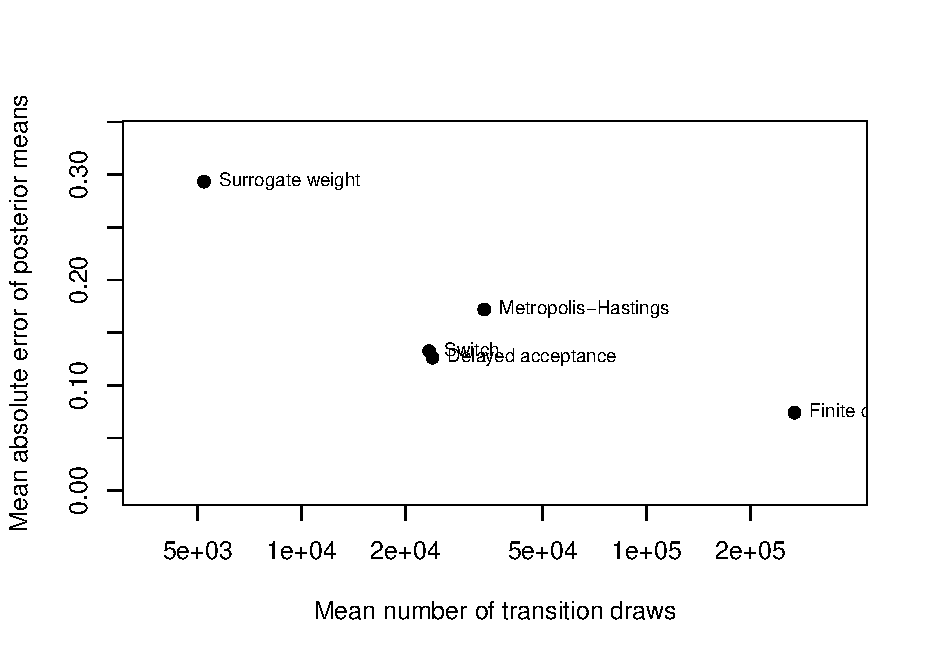
\includegraphics[width=0.85\textwidth]{figures/cost-error.pdf}
\caption{Mean absolute error of the posterior means of \(\log\theta_i\) against the mean number of transition draws. The finite-difference proposal is shown as a comparison that is not retained. Source: \texttt{summary-s2.csv}, \texttt{summary-s3.csv} and \texttt{summary-s4.csv}.}
\label{fig:cost}
\end{figure}

Figure~\ref{fig:cost} places the same runs on one scale, together with the surrogate-weight filter and the finite-difference proposal. The finite-difference proposal had mean absolute error 0.074 and mean transition draws 268602, against 0.172 and 33855 for the random walk. Effective sample size per transition draw was 0.000148 against 0.00123. The proposal does not improve that ratio. We do not retain it. The acceptance probability included the Gaussian proposal density, so the negative result is about cost, not about leaving \(\hat{\pi}_{\mathrm{enkf}}\).

The surrogate-weight filter used 5217 transition draws on average. The mean of the median absolute log differences between the surrogate increment and a fresh ensemble Kalman increment was 0.277, below the threshold of 1. The mean absolute error was 0.293, larger than the error of the plain filter and of delayed acceptance. The cost falls because most particles do not run a forecast. The target is \eqref{eq:knn-target}. The larger error is the visible part of the second approximation.

\begin{table}[t]
\centering
\caption{Sample variance of the log ensemble Kalman likelihood at the true parameter, from 20 independent ensembles. Source: \texttt{s5-variance.csv}.}
\label{tab:s5}
\begin{tabular}{rrrr}
\hline
\(d_y\) & \(N\) & Variance & Mean draws \\
\hline
1 & 8 & 14.060 & 128 \\
1 & 16 & 2.879 & 256 \\
5 & 8 & 24.935 & 640 \\
5 & 16 & 10.661 & 1280 \\
\hline
\end{tabular}
\end{table}

Table~\ref{tab:s5} is the scaling check that this pilot can support. The five-dimensional series is five independent copies of the same diffusion, with independent observation noise. Doubling \(N\) reduces the variance in both rows. The variance does not scale by the ratio of the observation dimensions. \citet[Proposition~2]{katzfuss2018} assumes independent draws from the true forecast in a different example. The ensemble used here is interacting, and the log-likelihood is a sum over the series. We do not draw a boundary at parameter dimension 10 or observation dimension 10.

\begin{table}[t]
\centering
\caption{Rao-Blackwellised weights. The identity row uses \(R_g = R = 0.1\). The other two rows use \(R_g = 0.5\) whilst the data and the gold standard use \(R = 0.1\). Error per draw is the ratio of the two means. Source: \texttt{summary-s6.csv} and \texttt{s6-identity.csv}.}
\label{tab:s6}
\begin{tabular}{lrrr}
\hline
Filter & Abs.\ error & Draws & Error per draw \\
\hline
Plain, \(R_g = 0.5\) & 0.369 & 22776 & \(1.62 \times 10^{-5}\) \\
Rao-Blackwellised, \(R_g = 0.5\) & 0.169 & 36069 & \(4.68 \times 10^{-6}\) \\
Rao-Blackwellised, \(R_g = 0.1\) & 0.121 & 31248 & \(3.87 \times 10^{-6}\) \\
\hline
\end{tabular}
\end{table}

When \(R_g = R\), the maximum absolute difference between the log ensemble Kalman increment and the log Rao-Blackwellised increment was 0 on each replicate. The correction does not change the weight. When \(R_g = 0.5\) and the true observation variance is 0.1, both densities are Gaussian and \(f \ne g\). The Rao-Blackwellised filter then has the smaller error per draw. That comparison is not a nonlinear observation model, and SMC2 was not run.

\section{Discussion}
\label{sec:disc}

The nested ensemble Kalman filter keeps an SMC2 recursion in problems where an unbiased particle likelihood is too expensive, at the cost of targeting \(\hat{\pi}_{\mathrm{enkf}}\) rather than the exact posterior. On the linear Gaussian pilot, delayed acceptance, the time switch and the Rao-Blackwellised identity behave as the arguments in Section~\ref{sec:methods} suggest, and the finite-difference proposal does not earn its cost.

Delayed acceptance, with the neighbour surrogate corrected by the ensemble Kalman likelihood, reduced the number of transition draws relative to a plain random walk and also reduced the absolute error, on this example. An exact tree returned the same neighbour sets as a list. It evaluated fewer distances at parameter dimension 3 and with 60 parameter particles. Whether that reduction remains once the tree is maintained, and whether it remains for a larger cloud, is open. The invariance argument above is for exact neighbours.

Choosing the plain kernel for the first half of the series, and delayed acceptance afterwards, lowered the cost per accepted move a little further than delayed acceptance alone. The rule is relatively ad hoc. Because it depends on the series only through time, the mixture of the two kernels preserves \(\hat{\pi}_{\mathrm{enkf}}\). A rule that looked at the proposed particle would sit inside the kernel, and no such rule was used.

The surrogate weight changes the target from \(\hat{\pi}_{\mathrm{enkf}}\) to \(\pi_{\mathrm{knn}}\). On the pilot the diagnostic stayed inside the threshold fixed in advance, the number of transition draws fell sharply, and the posterior means moved further from the gold standard than the means under \(\hat{\pi}_{\mathrm{enkf}}\). The surrogate weight is attractive only when that extra error is acceptable. A bound on the error is not available.

The Rao-Blackwellised correction leaves the weight unchanged when the observation model is already the linear Gaussian model inside the filter. The two log increments agreed exactly on the pilot. When the filter was run under a deliberately larger Gaussian variance, the correction reduced the error per draw. This is a narrow comparison between two Gaussian observation models. It does not establish the ordering, suggested by \citet{golightly2026}, of the plain nested filter, the Rao-Blackwellised filter and SMC2 under a nonlinear observation model.

The finite-difference proposal is the modification we drop. For linear transitions and a Gaussian initial law, a derivative of the ensemble Kalman log-likelihood converges to the true score as the ensemble grows \citep[Theorem~3.2]{chen2021}, and a Metropolis--Hastings correction can use a noisy finite difference without changing \(\hat{\pi}_{\mathrm{enkf}}\). Forming the difference, and the reverse density, repeated the filter often enough that the effective sample size per transition draw fell below that of the random walk. An uncorrected Langevin proposal was not used.

The pilot has several limits of its own. The gold-standard chain is short, the parameter dimension is three, and the observation dimension in the main comparison is one. Table~\ref{tab:s5} is the only step towards the regime suggested by \citet{golightly2026}, and it does not confirm a threshold there. The Gamma priors were given a shape-rate reading that the source paper does not state. The series are simulated. The comparisons above already use a model with a known likelihood.

What remains open is a bound on the discrepancy between \(\pi_{\mathrm{knn}}\) and \(\hat{\pi}_{\mathrm{enkf}}\), a neighbour search whose wall-clock cost is measured at the cloud sizes used in applications and a nonlinear observation model on which the Rao-Blackwellised weight can be compared with SMC2.


\bibliographystyle{apalike}
\bibliography{references}

\end{document}
